\documentclass{article}
\usepackage[utf8]{inputenc}
\usepackage[usenames,dvipsnames,svgnames,table]{xcolor}
\usepackage{amsmath,amsfonts}
\usepackage{lmodern}
\usepackage{graphicx}  % permet l'insertion d'images
\usepackage[left=2cm,right=2cm,top=2cm,bottom=2cm]{geometry}

% Définition des symboles
\newcommand{\N}{\mathbb{N}} % \N pour les entiers naturels
\newcommand{\R}{\mathbb{R}} % \R pour les réels
\newcommand\V[1]{\overrightarrow{#1}} % $\V{AB}$ pour les vecteurs

\title{TRAITEMENT D'IMAGE\\Débruitage}
\author{Adrien MARQUÈS - Alexis HELSON }
\date{Septembre 2015}

\begin{document}

	\maketitle
	
	% ======================== %
	% === PART 1 - PRELUDE === %
	% ======================== %
	\part*{Prélude}
		
		% ====================== %
		% === SECT 1 - INTRO === %
		% ====================== %
		\section{Introduction}
			De nombreuses images numériques sont produites aujourd'hui : imagerie médicales, images grand public (appareils photos numériques), numérisation de films ancienc, etc... Une problématique qui se pose est le débruitage des images obtenues. Nous proposons dans ce dossier d'aborder certaines techniques utilisées.\\
			\textbf{Image numérique}\par
			Une image numérique de taille \begin{math}n_{x} \times n_{y}\end{math} est composée de pixels (le nombre de pixels est \begin{math}n = n_{x}.n_{y}\end{math}), et pour chaque pixel on dispose (selon les cas) :\\
		 - une valeur entière comprise entre 0 et 255 (image en niveaux de gris codée en 8 bits)\\
		 - trois valeurs entières comprises entre 0 et 255, correspondant aux trois canaux de couleur (RGB)\\
		 - une valeur entière codée sur 12 ou 16 bits, ou même sur 1 seul, mais ces cas ne seront pas traités ici.\\
			\textbf{Bruit}\par
			Dans une image numérique, les processus de dégradation peuvent provenir de plusieurs sources, et donner du bruit qui peut avoir différentes expressions mathématiques. Notons \emph{u} l'image d'origine (l'image <<réelle>>) et \begin{math}u^{OBS}\end{math} l'image mesurée. Les exemples traités dans ce dossiers sont décrits ci-dessous.\par
			\indent{
				- l'image \begin{math}u^{OBS}\end{math} est mesurée par des appareils électroniques qui sont perturbés par des fluctuations aléatoires, et ces perturbations viennent s'ajouter au signal mesuré. On parle de \emph{bruit addifit}, et on a \begin{math}u^{OBS} = u + n,\end{math} où \emph{n} est le bruit ajouté.
			}\\
			\indent{
				- l'image \begin{math}u^{OBS}\end{math} comporte certains pixels où la valeur est aberrante (par exemple à cause d'un capteur défectueux, ou de défaut de transmission de l'information). Pour fixer les idées, on parle de \emph{bruit <<Salt and Pepper>>} lorsque certains pixels (au hasard) ont un niveau 0, et certains ont un niveau 255.
			}\\
			\indent{
				- lorsque le processus de formation de l'image comporte des compteurs de photons ou des photomultiplicateurs, lerreur commise peut être proportionnelle au signal mesurée. On parle alors de \emph{bruit multiplicatif} et on a \begin{math}u^{OBS} = u.(1+n)\end{math}.
			}\\
			
			
			\hrulefill\\
		
			Cette étude vise à améliorer les méthodes de \emph{nettoyage d'image}, et donc de développer un programme universel de débruitage, c'est-à-dire qu'il réduirait convenablement tout type de bruit, dépendant toutefois de paramètres adaptés à chacun.
			\begin{center} \emph{Avant d'essayer d'améliorer quelque chose, il faut d'abord le comprendre.} \end{center}
			Nous avons donc commencé par lire des études sur débruitage, la détection de contours, de formes, et la vectorisation d'images.
			\noindent Pour cela, nous avont étudié:
			\begin{description}
				\item[ - Le débruitage standard,]c'est à dire les méthodes déjà existantes.
				\item[ - Le filtrage par convolution,]afin de mettre en valeur les contours et formes et d'effectuer des "lissages".
				\item[ - La détection de formes,]afin d'effectuer un débruitage sans <<effet escalier>>.
				\item[ - La détection de contours,]afin d'optimiser la détection de formes.
			\end{description}
			Le programme a été développé en Python2 pour la simplicité et efficacité du langage. Le code est disponible sur Github à l'adresse suivante:
			\begin{center} \textcolor{blue}{https://github.com/xdrm-brackets/bmp\_python} \end{center}




		
		% =========================== %
		% === SECT 2 - ARCHI PROG === %
		% =========================== %
		\section{Architecture et structure du programme}
		
			\begin{figure}[!ht]
				\centering
				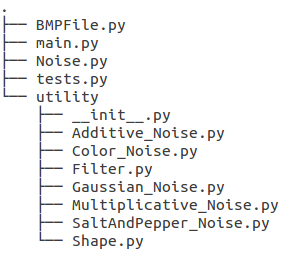
\includegraphics{fileTree.jpg}
			\end{figure}
		
			\begin{description}
				\item \textbf{main.py} \hfill \\
					Programme principal, il affiche une interface (en console) permettant d'éxécuter une des opérations disponibles.
				\item \textbf{tests.py} \hfill \\
					Contient les corps de toutes le opérations pouvant être choisies dans le programme principal.
				\item \textbf{BMPFile.py} \hfill \\
					Contient les structures \emph{BMPFile}, \emph{BMPContent}, \emph{BMPHeader}, permettant d'encoder et de décoder un fichier BMP. Ainsi que la strucure \emph{RGBPixel} permettant de coder un pixel.
				\item \textbf{Noise.py} \hfill \\
					Contient tout les traitements tels que les bruitages et débruitages, les filtres, et les détections de formes et contours. (il importe tout le dossier \emph{utility})
				\item \textbf{utility/}
				\begin{description}
					\item \textbf{SaltAndPepper\_Noise.py} \hfill \\
						Contient les méthodes de bruitage et débruitage du bruit de type \emph{Poivre \& Sel}.
					\item \textbf{Additive\_Noise.py} \hfill \\
						Contient les méthodes de bruitage et débruitage du bruit de type \emph{additif}.
					\item \textbf{Gaussian\_Noise.py} \hfill \\
						Contient les méthodes de bruitage et débruitage du bruit de type \emph{gaussien}.
					\item \textbf{Multiplicative\_Noise.py} \hfill \\
						Contient les méthodes de bruitage et débruitage du bruit de type \emph{multiplicatif}.
					\item \textbf{Color\_Noise.py} \hfill \\
						Contient les méthodes de bruitage et débruitage du bruit de type \emph{multicolore}.
					\item \textbf{Filter.py} \hfill \\
						Contient les méthodes de filtrage (standard et par convolution).
					\item \textbf{Shape.py} \hfill \\
						Contient les méthodes de détection de formes et de contours

				\end{description}
			\end{description}
		
			Le fichier \textbf{tests.py} utilise la structure \emph{BMPFile} afin de lire/écrire les fichiers ainsi que la structure \emph{Noise} qui contient toutes les méthodes de bruitage et de débruitage, les filtres et les détections de formes et de contours. Le fichier \emph{\textbf{Noise.py}} (qui contient la structure de même nom) appelle les différents fichiers contenus dans le dossier \textbf{utility}. Les fichiers contenus dans \textbf{utility} peuvent être:\\
			- Un fichier qui contient toutes les méthodes pour un type de bruit (bruitage et débruitage)\\
			- Le fichier \emph{Filters.py} qui contient toutes les méthodes de filtrage\\
			- Le fichier \emph{Shapes.py} qui contient toutes les méthodes de détection de formes et contours

	% ========================= %
	% === SECT 2 - VARIABLE === %
	% ========================= %
	\section{Variables globales}
		Ces valeurs seront utilisées pour la majeure partie des calculs et correspondent à des notations générales à l'image ou aux autres notations utilisées.\\\\
		\noindent
		Soit \begin{math}(n_x, n_y)\in\N^2\end{math}, respectivement la largeur et la hauteur de l'image en pixels.\\
		Soit la matrice \begin{math}I_{n_y, n_x}\end{math} correspondant à la répartition des pixels dans l'image.\\
		Soit le couple \begin{math}(x,y)\in\N^2\end{math}, les coordonnés d'un pixel dans I, tel que \begin{math}x\in[0;n_x[,\ et\ y\in[0;n_y[\end{math}.\\
		Soit \begin{math}\vec{u}\end{math} le vecteur associé à une unité de contour, tel que \begin{math}||\vec{u}|| = 1,\ et\ sa\ direction\ d =\frac{n\pi}{2}[2\pi]\ rad,\ avec\ n\in\N\end{math}.\\
		Soit \begin{math}K_n\end{math}, la matrice carré d'ordre \emph{n}. Par exemple \begin{math}K_3 = \begin{pmatrix}k_1&k_2&k_3\\k_4&k_5&k_6\\k_7&k_8&k_9\\\end{pmatrix}\end{math}\\\\


	\newpage


	
	% ========================= %
	% === PART 2 - ENCODAGE === %
	% ========================= %
	\part*{Encodage et décodage de fichiers}
		
		% =============================== %
		% === SECT 1 - FONCTIONNEMENT === %
		% =============================== %
		\section{Fonctionnement global}
			La lecture et l'écriture des fichiers se fait octet par octet, la structure \emph{BMPFile} permet de transformer les octets d'un fichier BMP en matrice de pixels, et inversement, de transformer une matrice de pixels en fichier BMP. Les types d'encodage des couleurs pris en charge sont 8 (nuance de gris), et 24 (rouge, vert, bleu) bits par pixels. Les pixels sont du type \emph{RGBPixel}, ce type contient les coordonnées du pixel (x, y), ainsi que sa couleur au format RGB (rouge, vert, bleu) chaque nuance prend sa valeur entre 0 et 255.
			\\\par Le seul format pris en charge est le format BMP. Pour que le programme fonctionne avec d'autres formats (jpeg, png, gif, etc), il suffirait de récupérer une matrice de \emph{RGBPixel} à partir d'une image. Toutes les méthodes de traitement d'image du programme agissent uniquement sur cette matrice. Il serait ainsi possible de convertir une image vers un autre format. Le fichier BMP peut se décomposer en 3 parties:
			\begin{description}
				\item - Le \emph{header} donne des informations sur le fichier et son contenu. \hfill\\
					Sa taille est de 54 octets.
				\item - La \emph{palette} donne des informations sur l'encodage des couleurs. \hfill\\
					Sa taille est variable, elle est donnée dans le header.
				\item - Le \emph{bitmap} est la matrice de pixels, c'est le <<corps>> du fichier. \hfill\\
					Sa taille est variable, elle est donnée dans le header.
			\end{description}
		
		
		% ====================== %
		% === SUBS 1 - HEADE === %
		% ====================== %
		\subsection{Le header}
			Le header fournit des informations sur le fichier, sur l'image, sur la palette et sur les tailles et positions des différentes parties. Il est
			\begin{center}\begin{tabular}{|c|c|l|}
				\hline \textbf{Position (octets)} & \textbf{Taille} & \textbf{Libellé}\\
				\hline 0  & 2 octets & signature, toujours 4D42\\
				\hline 2  & 4 octets & taille du fichier (octets)\\
				\hline 6  & 2 octets & réservé (défaut: 0)\\
				\hline 8  & 2 octets & réservé (défaut: 0)\\
				\hline 10 & 4 octets & offset de la bitmap (octets)\\
				\hline 10 & 4 octets & taille du BITMAPINFOHEADER (octets)\\
				\hline 14 & 4 octets & largeur de l'image (pixels)\\
				\hline 18 & 4 octets & hauteur de l'image (pixels)\\
				\hline 22 & 2 octets & nombre de plans (défaut: 0001)\\
				\hline 26 & 2 octets & nombre de bits par pixels (1, 4, 8, ou 24)\\
				\hline 30 & 4 octets & type de compression (0=rien, 1=RLE-8, 2=RLE-4)\\
				\hline 34 & 4 octets & taille de l'image padding inclus (octets)\\
				\hline 38 & 4 octets & résolution horizontale (pixels)\\
				\hline 42 & 4 octets & résolution verticale (pixels)\\
				\hline 46 & 4 octets & nombre de couleurs ou 0\\
				\hline 50 & 4 octets & nombre de couleurs importantes ou 0\\
	
				\hline
			\end{tabular}\newline\newline Figure 1 - BMP Header\end{center}
		
		% ====================== %
		% === SUBS 2 - PALET === %
		% ====================== %
		\subsection{La palette}
		La palette permet de définir les différentes couleurs d'une image. Elle correspond à une liste de couleurs ou bien à un <<code>> associé à un encodage spécifique. Elle dépend en premier lieu du nombre de bits par pixels. Cette valeur nous informe sur combien de bits est codée chaque couleur, les valeurs possibles sont 1, 4, 8, et 24. Le nombre de couleurs possibles dépend directement du \emph{bpp} (bits par pixels), plus il est grand, plus il y a de nuances. \begin{math}nbcouleurs = 2^{bpp}\end{math}. Les différents types de palette correspondant à un \emph{bpp} sont décrites ci-dessous.
		
			% ======================== %
			% === S2SECT 1 - 8 BPP === %
			% ======================== %
			\subsubsection{Encodage en 8 bits par pixels}
			Pour une image encodée en 8 bits par pixels, chaque pixel est codé sur 1 octet. Il y a donc une possibilité de \begin{math}2^8 = 256\end{math} couleurs. Ces 256 couleurs sont définies dans la \emph{palette} sur 4 octets chacunes. Les 3 premiers octets contiennent les couleurs au format RGB, et le dernier octet est à "0", c'est un octet de bourrage car la taille du fichier doit être multiple de 4. Par exemple si l'on veut que la couleur "0" corresponde à du rouge (R=255,G=0,B=0), et la couleur 1 à du rose (R=255,G=0,B=255), la palette commencera par: \\\\
			\begin{tabular}{|c|c|c|c|c|c|}
				\hline
				\textbf{rang}&\textbf{couleur}&\textbf{octet1}&\textbf{octet2}&\textbf{octet3}&\textbf{octet4}\\\hline
				0   & rouge & 255 & 0  & 0   & 0\\\hline
				1   & rose  & 255 & 0  & 255 & 0\\\hline
				..  & ..    & ..  & .. & ..  & ..\\\hline
				255 & ..    & ..  & .. & ..  & 0\\\hline
			\end{tabular}\\\\
			Par défaut, nous utilisons uniquement le codage en 8 bits par pixels pour des nuances de gris, notre palette a donc comme valeurs:\\\\
			\begin{tabular}{|c|c|c|c|c|c|}
				\hline
				\textbf{rang}&\textbf{couleur}&\textbf{octetS}&\textbf{octet2}&\textbf{octet3}&\textbf{octet4}\\\hline
				0   & noir  & 0   & 0   & 0   & 0\\\hline
				1   & noir  & 1   & 1   & 1   & 0\\\hline
				2   & noir  & 2   & 2   & 2   & 0\\\hline
				..  & ..    & ..  & ..  & ..  & ..\\\hline
				254 & blanc & 254 & 254 & 254 & 0\\\hline
				255 & blanc & 255 & 255 & 255 & 0\\\hline
			\end{tabular} * \begin{math}4\times256 = 1024\ octets\end{math} au total
	
	
			% ========================= %
			% === S2SECT 2 - 24 BPP === %
			% ========================= %
			\subsubsection{Encodage en 24 bits par pixels}
			Pour une image encodée en 24 bits par pixels, chaque pixel est codé sur 3 octets au format BGR, ce format est équivalent au format RGB, mis à part l'ordre des octets qui est inversé, celà correspond à \begin{math}2^24 = 16.777.216\end{math} couleurs par pixels. La \emph{palette} associée est définie par défaut comme suit:\\\\
			\begin{tabular}{|c|c|c|c|}
				\hline
				\textbf{Position (octets)}&\textbf{Taille (octets)}&\textbf{Valeur entière}&\textbf{Valeur ASCII}\\\hline
				0  & 1  & 66  & "B" \\\hline 
				1  & 1  & 71  & "G" \\\hline 
				2  & 1  & 82  & "R" \\\hline 
				3  & 1  & 115 & "s" \\\hline 
				4  & 48 & 0   & inconnu\\\hline 
				52 & 1  & 2   & inconnu\\\hline 
				53 & 15 & 0   & inconnu \\\hline 
			\end{tabular} * 68 octets au total
		
		
		% ====================== %
		% === SUBS 3 - BITMA === %
		% ====================== %
		\subsection{Le bitmap}
	
		Le \emph{bitmap} du fichier (matrice de pixels) peut avoir plusieurs formats qui sont propres au nombre de bits par pixels et dépendent de la \emph{palette}. De plus la matrice est dans l'ordre inverse, c'est à dire que le premier pixel est en fait le dernier, il convient donc d'inverser les lignes et les colonnes. De manière générale les pixels sont enregistrés en une succession de lignes. Le nombre d'octets de chaque ligne doit être un multiple de 4, est donc ajouté en fin de ligne un <<padding>> composé de 0 à 3 octets ayant pour valeur zéro.
	
	
		
	
	
	
	\newpage
	
	
	
	
	
	% ====================== %
	% === PART 3 - BRUIT === %
	% ====================== %
	\part*{Bruits}
	
	
	
	
		% =================== %
		% === SECT1 - P&S === %
		% =================== %
		\section{Le bruit de type <<Poivre \& Sel>>}
		\textbf{Définition graphique: }L'image est parsemée de pixels ayant une teinte extrême (blancs ou noirs) sans rapport avec leur contexte (voisinage).\\\\
		\textbf{Bruitage: }Le bruitage se fait en fonction du paramètre réel \begin{math}seuil\in[0;1]\end{math}. Il y a donc \begin{math}n = seuil\times width\times height\end{math} couples \begin{math}(x, y)\end{math} aléatoires qui sont en noir ou blanc (choix aléatoire), ce qui correspond à \begin{math}(100\times seuil)\end{math} \% de la totalité des pixels.\\\\
		\textbf{Débruitage: }L'image est débruitée en fonction de deux paramètres \emph{seuil} et \emph{borne}, tout deux compris dans \begin{math}[0;255]\end{math}. Chaque pixel est traité si et seulement si il est proche du noir ou du blanc, c'est-à-dire compris dans \begin{math}[0;borne]\end{math} pour le noir et dans \begin{math}[255-borne;255]\end{math} pour le blanc. Chaque pixel traité est comparé à la couleur moyenne de ses 8 voisins, si la différence avec sa couleur est supérieure à \emph{seuil}, le pixel se voit attribuer la couleur moyenne de ses voisins. Il est à noter que si borne vaut 255, tout les pixels seront traités, de même que si seuil vaut 255, tout les pixels traités se verront affecter la couleur moyenne de leurs voisins.\\\\
		% effet 50%
		\begin{figure}[!ht]
			\centering
			\begin{minipage}[t]{3.5cm}
				\centering
				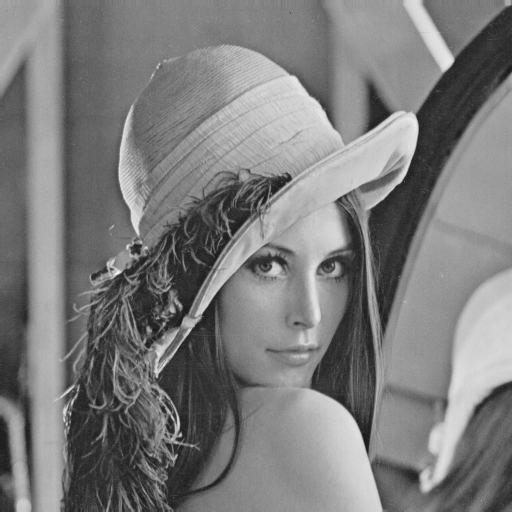
\includegraphics[width=3.5cm,height=3.5cm]{lena.jpg}
				Image originale
			\end{minipage}
			\begin{minipage}[t]{3.5cm}
				\centering
				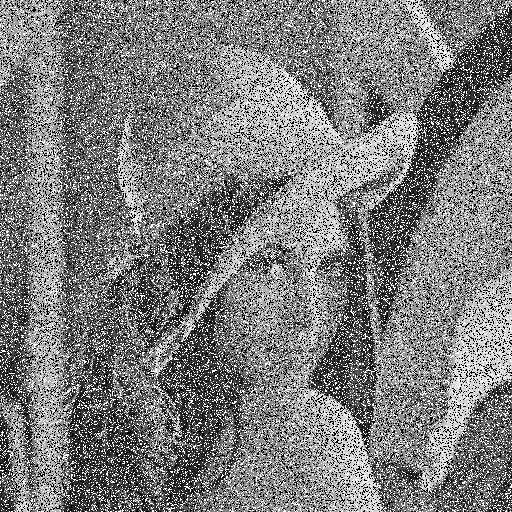
\includegraphics[width=3.5cm,height=3.5cm]{SaltAndPepper/noisy_50.jpg}
				Bruitée, seuil de 0.5
			\end{minipage}
			\begin{minipage}[t]{3.5cm}
				\centering
				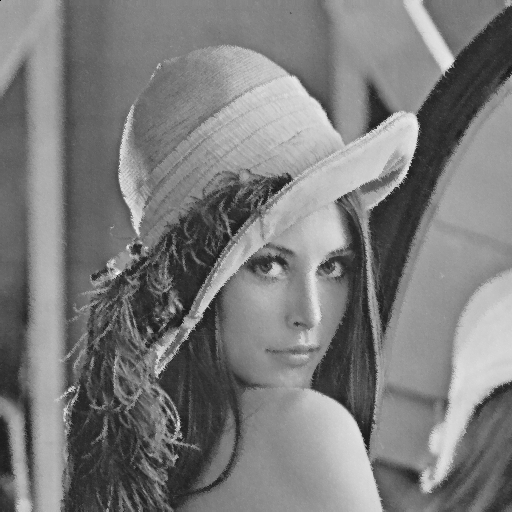
\includegraphics[width=3.5cm,height=3.5cm]{SaltAndPepper/algo1_50.jpg}
				Débruitée sans lissage
			\end{minipage}
			\begin{minipage}[t]{3.5cm}
				\centering
				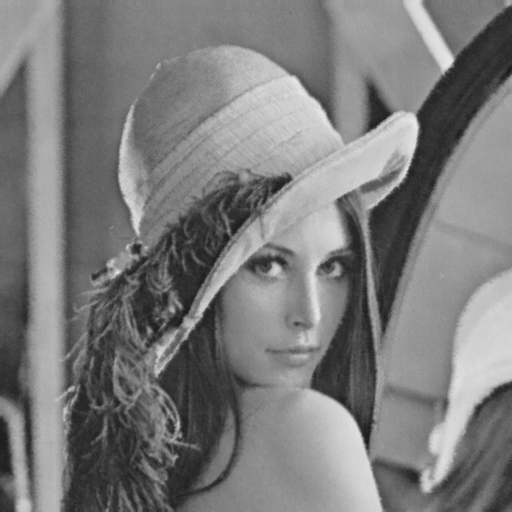
\includegraphics[width=3.5cm,height=3.5cm]{SaltAndPepper/algo2_50.jpg}
				Débruitée avec lissage
			\end{minipage}
		\end{figure}
		
		% effet 50% (zoom)
		\begin{figure}[!ht]
			\centering
			\begin{minipage}[t]{3.5cm}
				\centering
				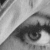
\includegraphics[width=3.5cm,height=3.5cm]{lenaZOOM.jpg}
				Image originale (zoom)
			\end{minipage}
			\begin{minipage}[t]{3.5cm}
				\centering
				
\includegraphics[width=3.5cm,height=3.5cm]{SaltAndPepper/noisy_50_ZOOM.jpg}
				Bruitée, seuil de 0.5 (zoom)
			\end{minipage}
			\begin{minipage}[t]{3.5cm}
				\centering
				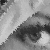
\includegraphics[width=3.5cm,height=3.5cm]{SaltAndPepper/algo1_50_ZOOM.jpg}
				Débruitée sans lissage (zoom)
			\end{minipage}
			\begin{minipage}[t]{3.5cm}
				\centering
				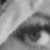
\includegraphics[width=3.5cm,height=3.5cm]{SaltAndPepper/algo2_50_ZOOM.jpg}
				Débruitée avec lissage (zoom)
			\end{minipage}
		\end{figure}
		On remarque bien ici que les contours subissent un <<effet escalier>> ce qui dégrade en majeure partie le rendu. Nous avons réglé partiellement ce problème en ajoutant un lissage au processus de débruitage, mais le lissage réduit aussi la netteté de l'image. Par contre, les couleurs sont convenablement restituées, de même pour les teintes et contrastes. Il suffirait de traiter l'image en prenant en compte les contours, ce qui permettrait de gagner en qualité.

	\newpage
	
	
		% =================== %
		% === SECT2 - BER === %
		% =================== %
		\section{Le bruit additif de Bernouilli}
		\textbf{Définition graphique: }L'image est parsemée de pixels ayant une teinte plus ou moins incohérente avec leurs contexte (voisinage). Ceci ressemble au bruit <<Poivre et Sel>> mais les pixels ne sont pas uniquement blancs ou noirs, mais parfois plus proches de la teinte d'origine.\\\\
		\textbf{Bruitage: }Le bruitage se fait en fonction du paramètre réel \begin{math}seuil\in[0;1]\end{math}. Il y a donc \begin{math}n = seuil\times width\times height\end{math} couples \begin{math}(x, y)\end{math} aléatoires qui voient leur couleur changée (choix aléatoire), ce qui correspond à \begin{math}(100\times seuil)\end{math} \% de la totalité des pixels. Soit un pixel aléatoirement choisi de couleur \begin{math}c \in [0;255]\end{math}. Soit:\\
		- sa teinte reste inchangée, mais il est éclairci (plus ou moins)\\
		- sa teinte reste inchangée, mais il est foncé (plus ou moins)\\\\
		\textbf{Débruitage \begin{math}\textbf{n}^\textbf{o}\end{math}1: }L'image est débruitée en fonction du paramètre \begin{math}seuil \in [0;255]\end{math}. Chaque pixel traité est comparé à la couleur moyenne de ses 8 voisins, si la différence avec sa couleur est supérieure à \emph{seuil}, le pixel se voit attribuer la couleur moyenne de ses voisins. Il est à noter que si seuil vaut 255, tout les pixels traités se verront affecter la couleur moyenne de leurs voisins.\\\\
		% effet 50%
		\begin{figure}[!ht]
			\centering
			\begin{minipage}[t]{5cm}
				\centering
				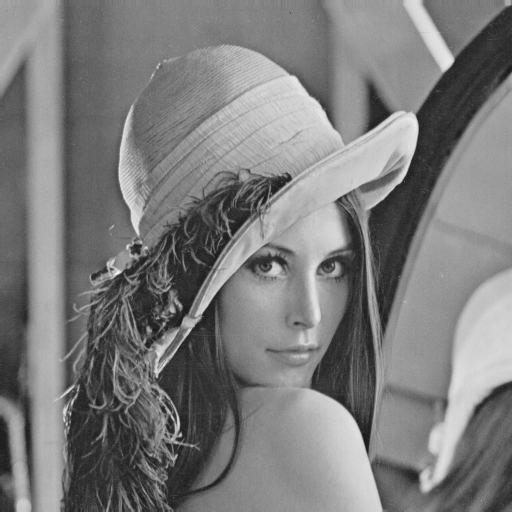
\includegraphics[width=5cm,height=5cm]{lena.jpg}
				Image originale
			\end{minipage}
			\begin{minipage}[t]{5cm}
				\centering
				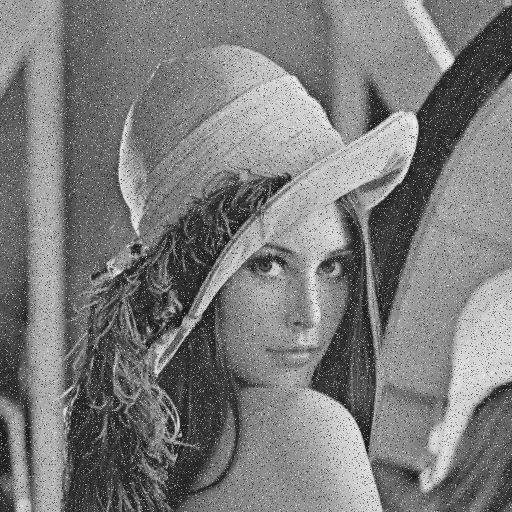
\includegraphics[width=5cm,height=5cm]{Additive/noisy_30.jpg}
				Bruitée, seuil de 0.3
			\end{minipage}
			\begin{minipage}[t]{5cm}
				\centering
				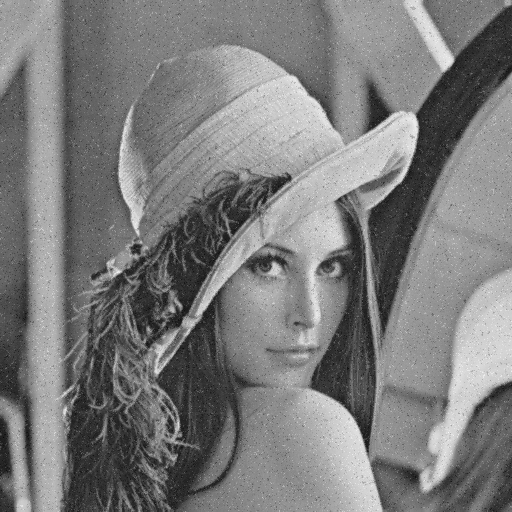
\includegraphics[width=5cm,height=5cm]{Additive/algo1_30.jpg}
				Débruitée, seuil de .35
			\end{minipage}
		\end{figure}
		
		% effet 50% (zoom)
		\begin{figure}[!ht]
			\centering
			\begin{minipage}[t]{5cm}
				\centering
				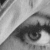
\includegraphics[width=5cm,height=5cm]{lenaZOOM.jpg}
				Image originale (zoom)
			\end{minipage}
			\begin{minipage}[t]{5cm}
				\centering
				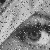
\includegraphics[width=5cm,height=5cm]{Additive/noisy_30_ZOOM.jpg}
				Bruitée, seuil de 0.3 (zoom)
			\end{minipage}
			\begin{minipage}[t]{5cm}
				\centering
				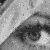
\includegraphics[width=5cm,height=5cm]{Additive/algo1_30_ZOOM.jpg}
				Débruitée, seuil de .35 (zoom)
			\end{minipage}
		\end{figure}
		On remarque bien ici qu'une majorité des pixels ajoutés lors du bruitage a été proprement retirée, mais une partie reste bien visible. Celà est du au fait que les pixels considérés comme bruit se voient appliquer un filtre moyen (couleur moyenne des voisins), mais que certains voisins peuvent être eux-aussi corrompus. De plus, certains pixels corrompus ne sont pas traités du fait qu'ils ont une teinte trop proche de la moyenne voisine. Il faut noter que lors du débruitage <<Poivre et Sel>> le paramètre \emph{borne} permettait d'éviter ce problème car nous avions des références absolues : le noir et le blanc. Nous avons donc décidé d'améliorer cet algorithme de débruitage (cf. \emph{Débruitage \begin{math}n^o\end{math}2}).\\\\
		
		
		\newpage
		
		
		\textbf{Débruitage \begin{math}\textbf{n}^\textbf{o}\end{math}2: }L'image est débruitée en fonction du paramètre \begin{math}seuil \in \N^+ \text{, tel que } seuil \in [0; \frac{n^2-1}{2} ] \end{math}. Pour chaque pixel, on établit la matrice carré \begin{math}M_n\end{math} d'ordre \emph{n} correspondant à son voisinage. Soit \begin{math}P_{2,2}\end{math} le pixel en cours, et
		 \begin{align*}M_{3} = \begin{pmatrix}
			P_{1,1} & P_{1,2} & P_{1,3}\\
			P_{2,1} & P_{2,2} & P_{2,3}\\
			P_{3,1} & P_{3,2} & P_{3,3}\\
		\end{pmatrix}\end{align*}
		
		\noindent On calcule ensuite \begin{math}M'_n\end{math} la matrice carré d'ordre \emph{n} correspondant à la différence absolue à \begin{math}P_{2,2}\end{math}.
		\begin{align*}
			M'_3 =
			\begin{pmatrix}
				|P_{1,1}-P_{2,2}| & |P_{1,2}-P_{2,2}| & |P_{1,3}-P_{2,2}|\\
				|P_{2,1}-P_{2,2}| & |P_{2,2}-P_{2,2}| & |P_{2,3}-P_{2,2}|\\
				|P_{3,1}-P_{2,2}| & |P_{3,2}-P_{2,2}| & |P_{3,3}-P_{2,2}|\\
			\end{pmatrix}
			=
			\begin{pmatrix}
				|P_{1,1}-P_{2,2}| & |P_{1,2}-P_{2,2}| & |P_{1,3}-P_{2,2}|\\
				|P_{2,1}-P_{2,2}| & 0                 & |P_{2,3}-P_{2,2}|\\
				|P_{3,1}-P_{2,2}| & |P_{3,2}-P_{2,2}| & |P_{3,3}-P_{2,2}|\\
			\end{pmatrix}
		\end{align*}
		\noindent Soit \emph{m} les valeurs de \begin{math}M'_n\end{math} excepté \begin{math}P_{2,2}\end{math}  telles que \begin{math}m_i \leq m_{i+1}\end{math}, ce qui nous permet de calculer le \textbf{poids statistique} du pixel.
		\begin{align*}
			PS(P_{2,2}) = \sum_{i=0}^{\frac{n^2-1}{2}}{\ m_i}
		\end{align*}
		Si le poids statistique d'un pixel est supérieur à \emph{seuil}, alors un filtre moyen lui est appliqué.
		
		
		% effet 50%
		\begin{figure}[!ht]
			\centering
			\begin{minipage}[t]{5cm}
				\centering
				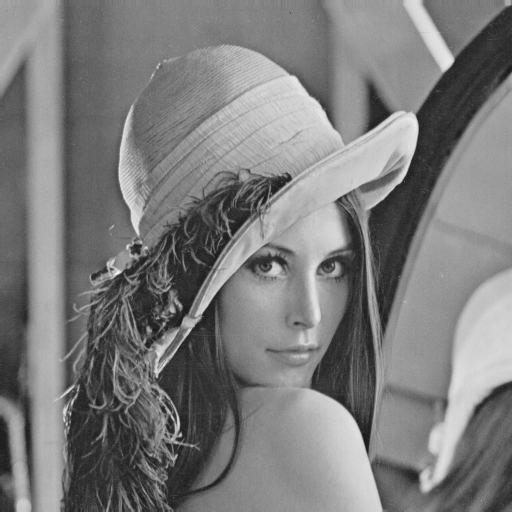
\includegraphics[width=5cm,height=5cm]{lena.jpg}
				Image originale
			\end{minipage}
			\begin{minipage}[t]{5cm}
				\centering
				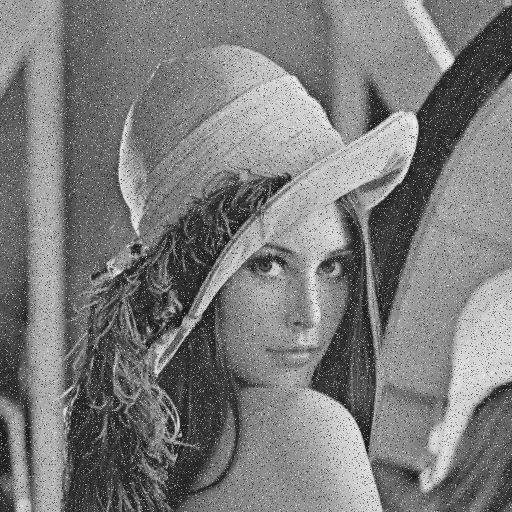
\includegraphics[width=5cm,height=5cm]{Additive/noisy_30.jpg}
				Bruitée, seuil de 0.3
			\end{minipage}
			\begin{minipage}[t]{5cm}
				\centering
				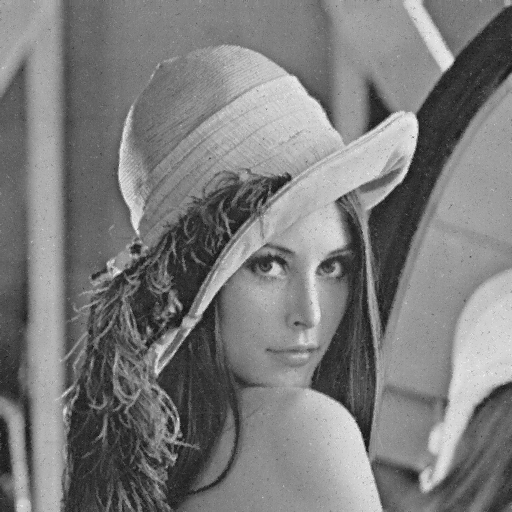
\includegraphics[width=5cm,height=5cm]{Additive/algo2_30.jpg}
				Débruitée, seuil de .05
			\end{minipage}
		\end{figure}
		
		% effet 50% (zoom)
		\begin{figure}[!ht]
			\centering
			\begin{minipage}[t]{5cm}
				\centering
				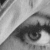
\includegraphics[width=5cm,height=5cm]{lenaZOOM.jpg}
				Image originale (zoom)
			\end{minipage}
			\begin{minipage}[t]{5cm}
				\centering
				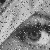
\includegraphics[width=5cm,height=5cm]{Additive/noisy_30_ZOOM.jpg}
				Bruitée, seuil de 0.3 (zoom)
			\end{minipage}
			\begin{minipage}[t]{5cm}
				\centering
				
\includegraphics[width=5cm,height=5cm]{Additive/algo2_30_ZOOM.jpg}
				Débruitée, seuil de .05 (zoom)
			\end{minipage}
		\end{figure}
		On remarque qu'avec cette nouvelle méthode, les contours sont moins dégradés et le bruit et d'autant plus diminué. Cet algorithme permet de différencier un contour d'un pixel bruité car la différence entre les poids statistiques écarte les deux cas.
	
	
	
		\newpage
		
		
	
		% =================== %
		% === SECT3 - ADD === %
		% =================== %
		\section{Le bruit additif gaussien}
		\textbf{Définition graphique: }Chaque pixel de l'image est plus ou moins bruitée, l'image semble avoir moins de contraste et chaque pixel est éclairci ou foncé.\\\\
		\textbf{Bruitage: }Le bruitage se fait en fonction du paramètre réel \begin{math}\sigma\in[0;255]\end{math}. Soit \emph{u} l'image d'origine, \begin{math}u^{OBS}\end{math} l'image observée et \emph{X} le bruit, on a :
		\begin{align*}
			u^{OBS} = u + X
		\end{align*}
		Afin de bruiter l'image, pour chaque pixel, on récupère un nombre réel \begin{math}r \in [0;1]\end{math} aléatoire, puis on applique la formule suivante:
		\begin{align*}
			u^{OBS}_{i,j} = u_{i,j} + r\sigma
		\end{align*}
		\textbf{Débruitage: }L'image est débruitée en fonction de deux paramètres \emph{seuil} et \emph{borne}, tout deux compris dans \begin{math}[0;255]\end{math}. Chaque pixel est traité si et seulement si il est proche du noir ou du blanc, c'est-à-dire compris dans \begin{math}[0;borne]\end{math} pour le noir et dans \begin{math}[255-borne;255]\end{math} pour le blanc. Chaque pixel traité est comparé à la couleur moyenne de ses 8 voisins, si la différence avec sa couleur est supérieure à \emph{seuil}, le pixel se voit attribuer la couleur moyenne de ses voisins. Il est à noter que si borne vaut 255, tout les pixels seront traités, de même que si seuil vaut 255, tout les pixels traités se verront affecter la couleur moyenne de leurs voisins.\\\\
		% effet 50%
		\begin{figure}[!ht]
			\centering
			\begin{minipage}[t]{3.5cm}
				\centering
				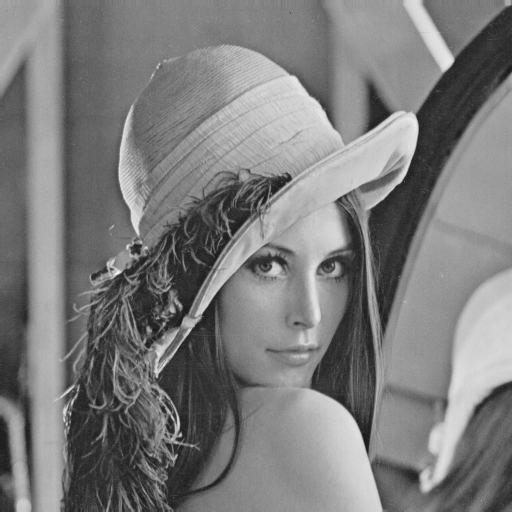
\includegraphics[width=3.5cm,height=3.5cm]{lena.jpg}
				Image originale
			\end{minipage}
			\begin{minipage}[t]{3.5cm}
				\centering
				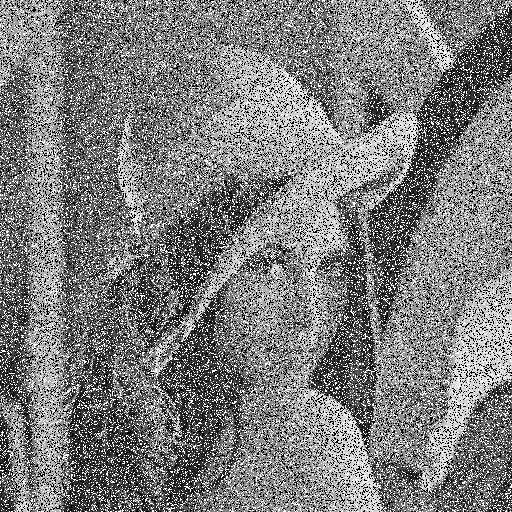
\includegraphics[width=3.5cm,height=3.5cm]{SaltAndPepper/noisy_50.jpg}
				Bruitée, seuil de 0.5
			\end{minipage}
			\begin{minipage}[t]{3.5cm}
				\centering
				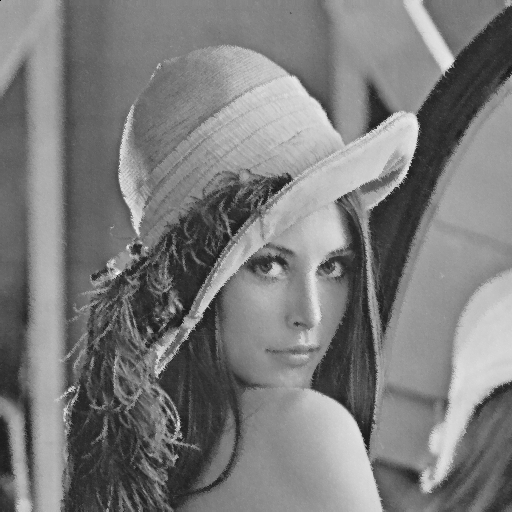
\includegraphics[width=3.5cm,height=3.5cm]{SaltAndPepper/algo1_50.jpg}
				Débruitée sans lissage
			\end{minipage}
			\begin{minipage}[t]{3.5cm}
				\centering
				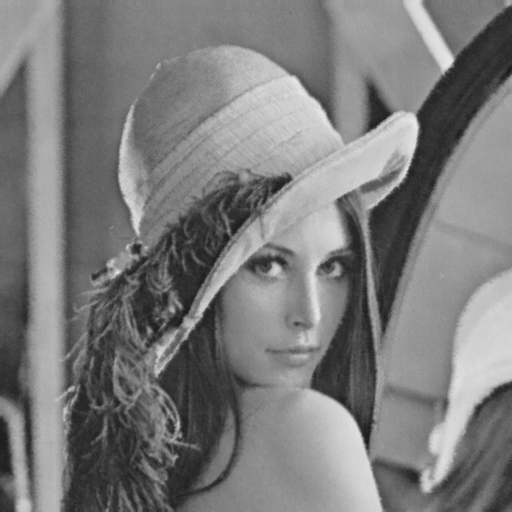
\includegraphics[width=3.5cm,height=3.5cm]{SaltAndPepper/algo2_50.jpg}
				Débruitée avec lissage
			\end{minipage}
		\end{figure}
		
		% effet 50% (zoom)
		\begin{figure}[!ht]
			\centering
			\begin{minipage}[t]{3.5cm}
				\centering
				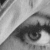
\includegraphics[width=3.5cm,height=3.5cm]{lenaZOOM.jpg}
				Image originale (zoom)
			\end{minipage}
			\begin{minipage}[t]{3.5cm}
				\centering
				
\includegraphics[width=3.5cm,height=3.5cm]{SaltAndPepper/noisy_50_ZOOM.jpg}
				Bruitée, seuil de 0.5 (zoom)
			\end{minipage}
			\begin{minipage}[t]{3.5cm}
				\centering
				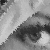
\includegraphics[width=3.5cm,height=3.5cm]{SaltAndPepper/algo1_50_ZOOM.jpg}
				Débruitée sans lissage (zoom)
			\end{minipage}
			\begin{minipage}[t]{3.5cm}
				\centering
				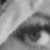
\includegraphics[width=3.5cm,height=3.5cm]{SaltAndPepper/algo2_50_ZOOM.jpg}
				Débruitée avec lissage (zoom)
			\end{minipage}
		\end{figure}
		On remarque bien ici que les contours subissent un <<effet escalier>> ce qui dégrade en majeure partie le rendu. Par contre, les couleurs sont convenablement restituées, de même pour les teintes et contrastes. Il suffirait de traiter l'image en prenant en compte les contours, ce qui permettrait de gagner en qualité.



	\newpage


	% ====================== %
	% === PART 4 - VECTO === %
	% ====================== %
	\part*{Vectorisation pour la détection de contours}
	
	
		% =================== %
		% === SECT1 - BAS === %
		% =================== %
		\section{Problème de base}
			\textbf{Problème: }Nous avons remarqué précedemment que de manière générale après un débruitage, les contours de l'image deviennent irréguliers.\\
			\textbf{Solution: }La solution retenue s'appuie sur la \textbf{vectorisation}, cette partie vise à <<régulariser>> les contours. Nous ne parlons pas ici de les lisser mais de les redessiner.\\
		
		
		% =================== %
		% === SECT2 - DET === %
		% =================== %
		\section{Processus détaillé}
			\textbf{Etape 1: }\par
			En premier lieu, il faut isoler les contours uniquement, il existe plusieurs moyens de le faire:\\
			- soustraire l'image de base à l'image lissée (filtre moyen)\\
			- utiliser un algorithme non-récursif d'indépendentisation de contour.\\
			Nous avons mis au point les 2 méthodes vues ci-dessus afin de comparer leur temps d'exécution et leur efficacité. Ceci nous permettra de plus de les combiner.\\
			
			\indent	\emph{Méthode 1 - soustraction de l'image lissée}\\
			L'image est lissée avec un filtre moyen. Nous effectuons un produit de convolution (noté \begin{math}\otimes\end{math}) avec l'image \emph{I} et le noyau tel que défini :
			\begin{align*}
				I_{lisse} = I\ \otimes\ \frac{1}{8} \begin{pmatrix}
					1 & 1 & 1\\
					1 & 0 & 1\\
					1 & 1 & 1
				\end{pmatrix} 
			\end{align*}
			On effectue ensuite la soustraction matricielle afin de mettre les contours en valeur\\
			
			\indent	\emph{Méthode 2 - indépendentisation de contour}\\
			Un algorithme lance sur chaque pixel de l'image un "envahisseur", c'est-à-dire un algorithme qui référencie chaque pixel considéré dans la même forme que le pixel de départ. par exemple, on obtient le résultat ci-dessous en essayant de récupérer les formes noires uniquement :
			% indépendentisation de contour 
			\begin{figure}[!ht]
				\centering
				\begin{minipage}[t]{3.5cm}
					\centering
					
\includegraphics[width=3.5cm]{Vectorization/shape.jpg}
					Image originale
				\end{minipage}
				\begin{minipage}[t]{3.5cm}
					\centering
					
\includegraphics[width=3.5cm]{Vectorization/shapeDetection1.jpg}
					Détection sur forme 1
				\end{minipage}
				\begin{minipage}[t]{3.5cm}
					\centering
					
\includegraphics[width=3.5cm]{Vectorization/shapeDetection2.jpg}
					Détection sur forme 2
				\end{minipage}
				\begin{minipage}[t]{3.5cm}
					\centering
					
\includegraphics[width=3.5cm]{Vectorization/shapeDetection3.jpg}
					Détection sur forme 3
				\end{minipage}
			\end{figure}\\
			Les résultats sont corrects mais le traitement devient vite très long, le temps d'éxécution moyen pour ces résultats est de 20 secondes. Nous avons donc décidé de créer un nouvel algorithme qui lui récupérerait uniquement les contours.
			
	
	\newpage
	
	
	
\end{document}